% 软件：CTeX套装v3.0.216.3：https://mirrors.tuna.tsinghua.edu.cn/ctex/3.0/
% 编译：XeLaTeX
% 编码：UTF-8
% 模板：淮安大学毕业设计（论文）
% 制作：刘绪庆
% 版本：v1.0

\documentclass[12pt,oneside]{../setup/hyit_S-2}

%++++++++++++++++++++++%
%                      %
% 自定义所需的其他宏包 %
%                      %
%----------------------%--------------------------------%
\usepackage[linesnumbered,ruled,vlined]{algorithm2e}
\let\algorithmuunderline\underline \def\underline{\relax}
\DontPrintSemicolon
\renewcommand{\algorithmcfname}{算法}
\SetKwInOut{KwIn}{输入}
\SetKwInOut{KwOut}{输出}
\crefname{algocf}{算法}{算法}
%+++++++++++++++++++++++++++++++++++++++++++++++++++++++%

%===========================================%
%             大论文的封面信息              %
%===========================================%
\def\YourName{某某某}        % 填写本人姓名 %
\def\YourNumber{12位数的学号}% 填写本人学号 %
\def\YourCollege{数理学院}   % 填写所在学院 %
\def\YourMajor{金融数学}     % 填写所学专业 %
\def\PaperTitleLa{标题第一行}% 标题的第一行 %
\def\PaperTitleLb{标题第二行}% 标题的第二行 %
\def\SupervisorNameIn{某某某}% 校内导师姓名 %
\def\SupervisorTitleIn{教授} % 校内导师职称 %
\def\SupervisorNameOut{/}    % 校外导师姓名 %
\def\SupervisorTitleOut{/}   % 校外导师职称 %
\def\MajorResp{某某某}       % 专业负责人   %
\def\PaperYear{2026}         % 完成时间(年) %
\def\PaperMonth{05}          % 完成时间(月) %
%===========================================%

% 中文摘要（仅修改 < > 部分）
\def\ChineseAbstract{%
  <中文摘要200-300字>
}

% 中文关键词（仅修改 < > 部分）：3-8个，全角逗号隔开，最后的关键词后不加标点
\def\ChineseKeywords{%
  <关键词1，关键词2，……>
}

% 英文标题（仅修改 < > 部分）：A第一行、B第二行
\def\EnglishTitleA{%
  <This is the First Line of the English Title>
}
\def\EnglishTitleB{%
  <This is the Second Line of the English Title>
}

% 英文摘要（仅修改 < > 部分）
\def\EnglishAbstract{%
  <This is the English abstract of the paper>
}

% 英文关键词（仅修改 < > 部分）：与中文关键词对应，一律小写
% 用“半角逗号+1个空格”隔开，最后的 keyword 后不加标点
\def\EnglishKeywords{%
  <keyword 1, keyword 2, ......>
}

% 总结与展望（仅修改 < > 部分）
\def\ConcludingRemark{%
  <总结课题完成了哪些相关工作，得到的成果如何（或得到了什么结论），
  相对于任务书要求，还存在哪些不足；可以提出建议、研究设想、改进
  思路、尚待解决的问题等等。
  >
}

% 致谢（仅修改 < > 部分）
\def\ThanksTo{%
  <本课题……>
}

\begin{document}
\FirstPage % 论文封面
\ChAbs     % 中文摘要
\EnAbs     % 英文摘要
\TocHeader % 论文目录
\MainFile  % 论文正文

%++++++++++++++++++++++++++++%
%                            %
% 使用 \section{} 创建“章” %
%                            %
%++++++++++++++++++++++++++++%
\section{引言}
\label{sec:Intro}
\par% 文本、交叉引用
本章……

图\ref{fig:clsFiles}、\cref{fig:clsFiles}、\autoref{fig:clsFiles}

表\ref{tab:toyExample}、\cref{tab:toyExample}、\autoref{tab:toyExample}

第\ref{sec:Intro}章、\cref{sec:Intro}

第\ref{subsec:Figure}节、\cref{subsec:Figure}

第\ref{subsubsec:Table}节、\cref{subsubsec:Table}

文献\cite{Authors2025}（上标位置）、文献\citeq{Authors2026}（水平位置）

算法\ref{algo:ToyExample}、\cref{algo:ToyExample}

%+++++++++++++++++++++++++++++++++%
%                                 %
% 使用 \subsection{} 创建二级标题 %
%                                 %
%+++++++++++++++++++++++++++++++++%
\subsection{图的示例}
\label{subsec:Figure}

\par% 图(一般不建议使用H，而是用!htbp)
\begin{figure}[H]
  \centering
  \fbox{%
    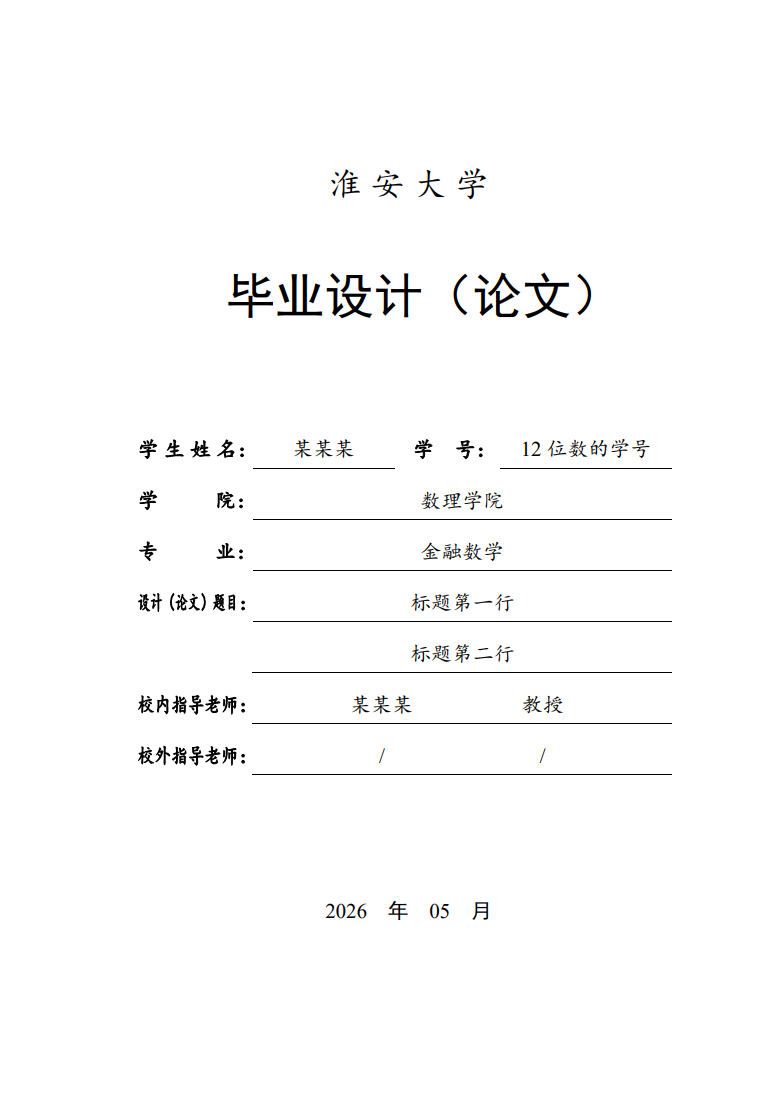
\includegraphics[width=0.5\textwidth]{RFs/PaperFirstPage.png}
  }
  \caption{淮安大学本科毕设模板文档}
  \label{fig:clsFiles}
\end{figure}

%++++++++++++++++++++++++++++++++++++%
%                                    %
% 使用 \subsubsection{} 创建三级标题 %
%                                    %
%++++++++++++++++++++++++++++++++++++%
\subsubsection{表格示例}
\label{subsubsec:Table}
\par% 表(一般不建议使用H，而是用!htbp)
\begin{table}[H]
  \centering
  \caption{表格标题在表格上方}
  \label{tab:toyExample}
  \begin{tblr}{
      colspec = {
        Q[b,c,wd=1.5cm]
        Q[b,c,wd=3.9cm]
        Q[b,c,wd=1.5cm]
      },
      colsep=6pt,
      row{1-Z} = {ht=0.4cm, abovesep=1pt, belowsep=1pt},
      hlines = {0pt}, hline{1,Z} = {1pt}, hline{2} = {0.5pt}, hspan = minimal,
      vlines = {0pt}, vline{1-Z} = {0pt}, vspan = minimal,
    }
    \textbf{\heitiBF 表头1} & \textbf{\kaishuBF 表头2} & \textbf{\songtiBF 表头3} \\
    数据11 & 数据12 & 数据13 \\
    数据21 & 数据22 & 数据23 \\
    数据31 & 数据32 & 数据33 \\
    数据41 & 数据42 & 数据43 \\
    数据51 & 数据52 & 数据53 \\
    数据61 & 数据62 & 数据63 \\
    数据71 & 数据72 & 数据73 \\
    数据81 & 数据82 & 数据83 \\
  \end{tblr}
\end{table}

%++++++++++++++++++++++++++++++++++++%
%                                    %
% 使用 \section{} 创建新的一个“章” %
%                                    %
%++++++++++++++++++++++++++++++++++++%
\section{算法示例}
\label{sec:Algo}
\par% 算法
这里是一个算法的伪代码：
\begin{algorithm}[!htbp]
\caption{此处为算法名}
\label{algo:ToyExample}
\KwIn{xxx}
\KwOut{yyy}
初始化zzz\;
\For{$i=0~\KwTo~10$}{
  \eIf{$j = 0$}{
    $k\gets 1$\;
  }{
    $\ell = 2$\;
  }
  \tcp{hahaha}
}
\Return{$i,j,k,\ell$}\;
\end{algorithm}

%++++++++++++++%
%              %
% “定义”环境 %
% “定理”环境 %
%              %
%++++++++++++++%
\section{定义、定理等环境的使用}
\label{sec:DefThm}

\par% 定义
\begin{definition}[<这里写定义的副标题>]
  设……，则称……
\end{definition}

\par% 定理
\begin{theorem}[<这里写定理的副标题>]
  若……，则……
\end{theorem}

\par% 证明
\begin{proof}
  由题意，知……
\end{proof}

\par

%++++++++++++%
%            %
% 总结与展望 %
%   致  谢   %
%            %
%++++++++++++%
\makeSummary
\makeAcknowledgement

%+++++++++++++++++++++++++++++++++++++++++%
%                                         %
% 使用 {thebibliography} 环境创建参考文献 %
%                                         %
% 1.原则上不少于20篇，其中外文不少于2篇； %
% 2.标点符号均应为“Times New Roman”格   %
%   式，且其后加1个空格；                 %
% 3.引用：\cite{} 或 \inlinecite{}        %
%                                         %
%+++++++++++++++++++++++++++++++++++++++++%
\begin{thebibliography}{99}
  \bibitem{Authors2025}
    作者1, 作者2. 论文标题[J], 期刊名, 2025(2): 167--173.
  \bibitem{Authors2026}
    作者1, 作者2. 论文标题[J], 期刊名, 2026(6): 109--123.
\end{thebibliography}

%++++++++++++%
%            %
%    附录    %
%            %
%++++++++++++%
\makeappendix
\subsection{问题1的MATLAB代码}
%\begin{matlab}
%\end{matlab}
\begin{lstlisting}[language=matlab,morekeywords={}]
function R = FV(D,x,k,m,n,idx,S)
switch m
    case {1,'pc'}
        for j = 1:x(k)-1
            n = n+1;
            for u = 1:length(idx)
                s = S(idx(u));
            end
        end
    case {2,'rk'} %省略
end
\end{lstlisting}

\end{document}
